% Fixed source PDF, printed page 49, question 23: schematic vector redraw.
% Edges/labels follow the source; spatial proportions are illustrative only.
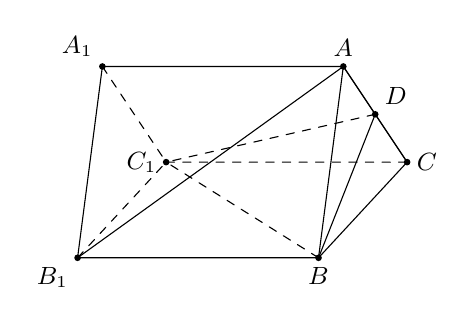
\begin{tikzpicture}[x=.9cm,y=.9cm,line cap=round,line join=round,font=\small]
  \coordinate (Aone) at (0,2.7);
  \coordinate (Bone) at (-.35,0);
  \coordinate (Cone) at (.9,1.35);
  \coordinate (A) at (3.4,2.7);
  \coordinate (B) at (3.05,0);
  \coordinate (C) at (4.3,1.35);
  \coordinate (D) at (3.85,2.025);

  % Prism edges and hidden edges as shown in the source schematic.
  \draw (Aone)--(A) (Aone)--(Bone) (Bone)--(B) (A)--(B)--(C)--cycle;
  \draw[dashed] (Aone)--(Cone) (Bone)--(Cone) (Cone)--(C);

  % The source-defined diagonals and plane DBC_1 used by the statements.
  \draw (Bone)--(A) (D)--(B);
  \draw[dashed] (B)--(Cone) (D)--(Cone);
  \draw (A)--(D)--(C);

  \fill (Aone) circle (1.2pt) (Bone) circle (1.2pt) (Cone) circle (1.2pt)
        (A) circle (1.2pt) (B) circle (1.2pt) (C) circle (1.2pt) (D) circle (1.2pt);
  \node[above left] at (Aone) {$A_1$};
  \node[below left] at (Bone) {$B_1$};
  \node[left] at (Cone) {$C_1$};
  \node[above] at (A) {$A$};
  \node[below] at (B) {$B$};
  \node[right] at (C) {$C$};
  \node[above right] at (D) {$D$};
\end{tikzpicture}
